\section{Modell}
Auf der Suche nach einem guten Modell für die Daten wurden mehrere Ansätze gewählt und verfeinert. Als Grundlage wurde sich an Modellen für die Lösung des MNIST-Datensatz (circa 70.000 handgeschrieben Ziffern) orientiert.  Dieser Datensatz ist öffentlich verfügbar und enthält insgesamt 70.000 Graustufen-Bilder von handgeschrieben Ziffern in 28 $\times$ 28 Pixel.  Er wird gerne als Beispiel für Einstieger verwendet.  \label{MNIST}
\subsection{Neuronales Netzwerk}
Es wurde als erstes Neuronales Netzwerk ein sequentielles Modell benutzt.  Dabei kann man mit Keras das Modell Schicht für Schicht aufbauen.\\
Das erste Modell besteht aus drei Schichten.\\
\lstinputlisting[language=Python,  firstline=24, lastline=28]{code/Modell.py}

Mit einer 'keras.layers.Dense' Schicht wird jedes Neuron einer Schicht mit jedem Neuron in der Nachbarschicht verbunden.  Als erstes wird die Anzahl der Neuronen in der Schicht festgelegt, danach ihre Aktivierungsfunktion und eine der möglichen weiteren Optionen beschreibt den Eingabevektor 'input\_shape'. \\
Der Eingabevektor von 9.296 entspricht einer Datengröße der Aufnahmen.  Die erste Schicht nach der Eingabe hat 2.000 Neuronen. Es soll die Anzahl der Faktoren reduziert werden damit der Ausgabevektor zum Schluss des Modells mit der Anzahl der Zielvariablen übereinstimmt. Als Aktivierungsfunktion wurde die Sigmoid-Funktion gewählt.  Die Sigmoid-Funktion gibt Werte zwischen Null und Eins zurück. 
\begin{equation}
sig(w,b) = \frac{1}{1+e^{\sum_{j} w_{j}z_{j} +b}}  \text{mit} j:= \text{ Neuron der Vorgängerschicht}
\end{equation}
Sie hat den Vorteil,  dass große Ausreißer in den Summe abgefangen werden mit ihrer Beschränktheit auf die Werte zwischen Eins und Null.  Außerdem ist sie einfach und stetig differenzierbar. Die Ableitung der Sigmoid-Funktion lässt sich auf sich selbst zurück führen.\\
\begin{equation}
sig(w,b)^{\prime} = sig(w,b)(1-sig(w,b)) \text{  \cite{Sigmoid2021}}
\end{equation}
Dieses erleichtert den Prozess des Lernens,  da der Computer dabei die Differenzialgleichung auflösen muss. \\
Für die letzte Schicht wurde ein Softmax-Aktivierungsfunktion gewählt. Diese Funktion hat die Eigenschaft, dass die Summe der Ergebnisse in der Ausgabe-Schicht Eins ist.  Also bekommt jedes Neuron als Ausgabe einen Wert zwischen Null und Eins. Gerade bei Klassifikationsaufgabe,  wie der in dieser Arbeit, kann damit eine Wahrscheinlichkeit, das eine Klasse richtig ist, bestimmt werden. \\
%Formel und Bild Erklärung, Matrix
Nachdem das Modell aufgebaut ist, wird im nächsten Schritt die Trainingsmethode festgelegt.  Dazu werden unter anderem die Verlustfunktion,  der Minimierungsprozess und die Lernrate bestimmt.
\lstinputlisting[language=Python,  firstline=40, lastline=42]{code/Modell.py}
Als Minimierungsprozess wurde die stochastischer Gradientenabstieg 'SGD' benutzt. Diese benutzt, wie in Kapitel \ref{Gradient} erklärt, den Gradienten für den Minimierungsprozess.  Bei dem stochastischen Gradientenabstieg wird in einer Trainingseinheit immer ein Datensatz zufällig (stochastische) ausgewählt, um den Gradient nur über diesen einen Datensatz zu bilden. Das hat den enormen Vorteil, dass extrem viel Zeit und Rechenleistung gespart wird besonders im Vergleich zu dem normalen Gradientenabstieg. Hierbei wird der Gradient für jeden Datensatz in der Trainingseinheit gebildet. \cite{Geron2019}\\
Der Nachteil des stochastischen Gradientenabstiegs  ist,  dass es durch den zufälligen ausgewählten Datensatz nie zum global Minimum kommt.  Bei einem hochdimensionalen Problem, wie die die durch Neuronale Netzwerke entstehen, gibt viele lokale Minima. Damit der Gradient sich besser an das  global Minimum nähert, werden Mini-Batches benutzt. Dadurch wird das Traingsset unterteilt und der stochastische Gradient in jedem dieser Stappel (Batch) gebildet. Dies führt zu weniger großen Sprüngen des Gradienten \cite{Geron2019}. \\
Die Lernrate wurde mehrfach angepasst um das Modell zu optimieren.  Die Verlustfunktion 'sparse\_categorical\_crossentropy' ist besonders nützlich für Klassifikationsaufgaben.  Es wird ein Eingabevektor nur einer möglichen Ziffer zuordnet.  Da es sich um eine Klassifikationsaufgabe handelt soll das Modell auf Genauigkeit evaluiert und trainiert werden, deswegen wurde 'metrics=['accuracy']' gewählt. \\
Danach wird das Modell trainiert, dazu müssen die Trainings- und Testdatensätze angegeben werden. Zusätzlich werden noch die Batch Größe und die Anzahl der Epochen festgelegt.
\lstinputlisting[language=Python,  firstline=44, lastline=56]{code/Modell.py}

Der Befehl 'print(history)' zeigt den Lernprozess des Algorithmus an.  Dieser kann außerdem in einer Graphik dargestellt werden.
\begin{figure}[h]
\centering
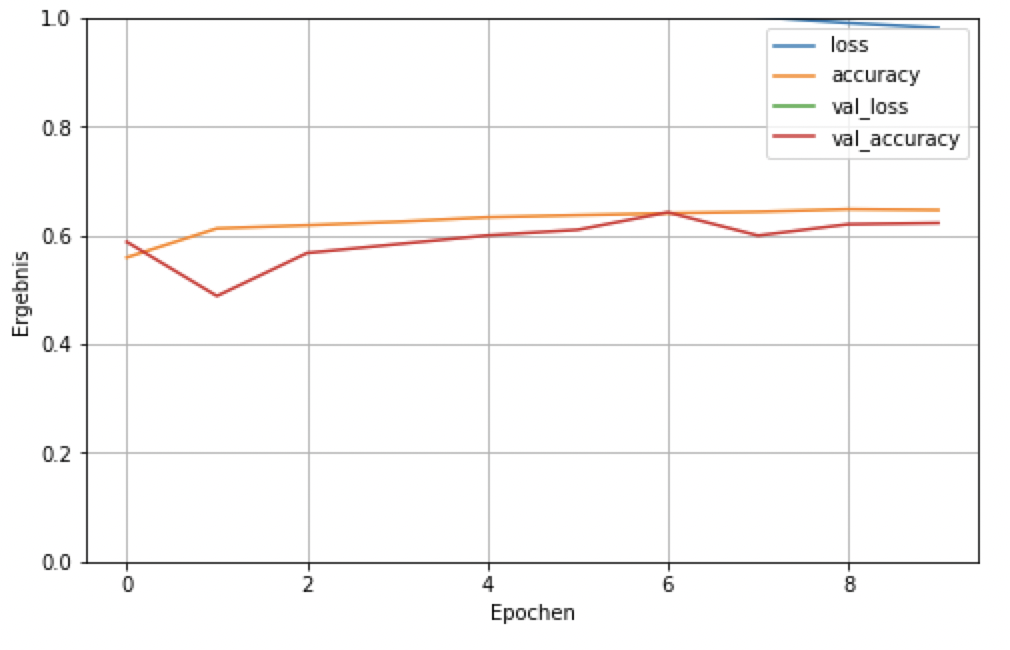
\includegraphics[scale=0.5]{pic/label000316}
\caption{Lernprozess bei Lernrate 0.003 Batch= 16}
\end{figure}
\subsubsection{Verbesserung}
Im ersten Modell ist die Genauigkeit nur langsam gestiegen. Daraus wurde angenommen, dass die Lernrate zu klein ist. Deswegen wurde als nächstes die Lernrate auf 0.005 erhöht. 
\begin{figure}[h]
\centering
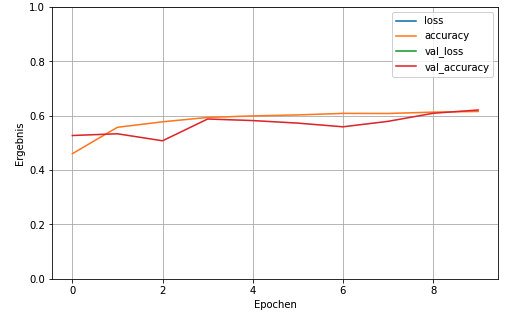
\includegraphics[scale=0.5]{pic/achse00516}
\caption{Lernprozess bei Lernrate 0.005 Batch= 16}
\end{figure}
Hier gab es stärker Schwankung bei der Genauigkeit der Testdaten.  Um zu überprüfen, ob die Lernphase einfach zu kurz war, wurde das ganze mit 30 anstelle von 10 Epochen wiederholt.
Nachdem auch dort nur langsame Lernfortschritte gemacht wurden,  wurde erneut versucht die Lernrate zu vergrößern.  Sie wurde auf 0.01 gesetzt.  Dies führt auch nicht zu einer deutlichen Verbesserung der Genauigkeit.\\
Als nächster Schritt wurde die Batch-Größe verkleinert auf 32.  Das heißt der Traingsdatenset wird in 32 Teilstücke unterteilt und nach jedem Lernen mit einem Batch werden die Parameter angepasst. 
\begin{figure}[h]
\centering
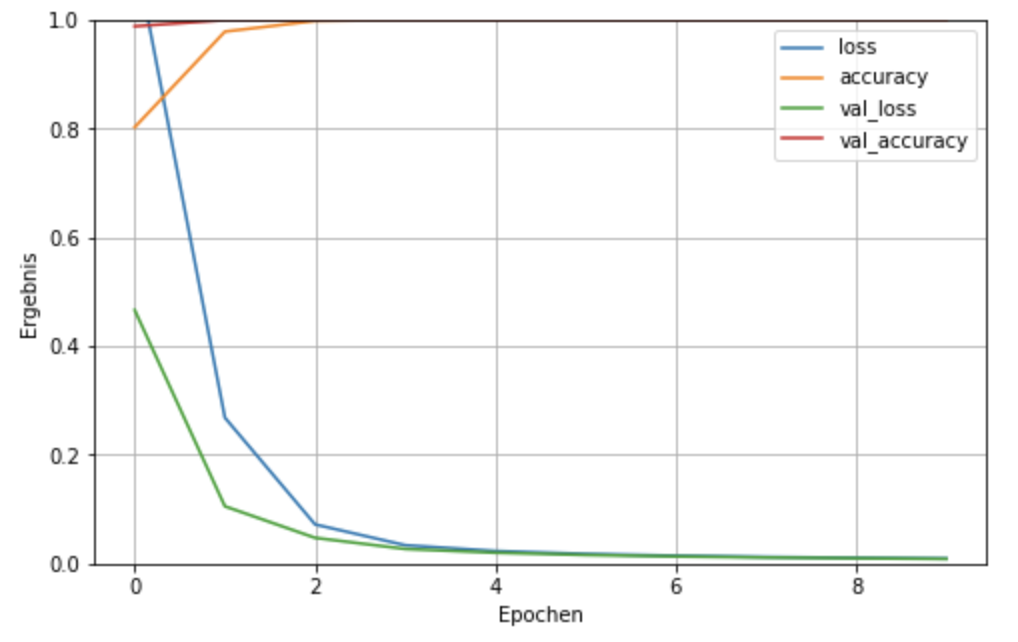
\includegraphics[scale=0.5]{pic/achsen00132}
\caption{Lernprozess bei Lernrate 0.01 Batch= 32}
\end{figure}
Das Unterteilen für zu schnelleren Veränderung der Parameter hat aber auch den Nachteil, dass es zu Overfitting führen kann.




\subsubsection{Überprüfung} \label{Überprüfung}
Zur Kontrolle, ob der Algorithmus nicht unwichtige Besonderheiten gelernt hat, wurde einzelne Bilder nochmals per Hand überprüft.\\
\begin{lstlisting}[language = Python]
test_model = tf.keras.models.load_model('drive/MyDrive/modelSeqSGD')
test_image = np.expand_dims(X_val[4], axis=0)
pre2 = test_model.predict(test_image)
pre2_max = np.argmax(pre2, axis = 1)
print('Image as Test. Label: {} Prediction {}'.format(y_val[4], pre2_max))
some_digit = X_val[4]
some_digit_image = some_digit.reshape(112,83)
plt.imshow(some_digit_image, cmap = mat.cm.binary, interpolation="nearest")
plt.axis("off")
plt.show()
\end{lstlisting}
Diese zeigten die Vorhersage und auch die Aufnahme wird dargestellt.
\begin{figure}[h]
\centering
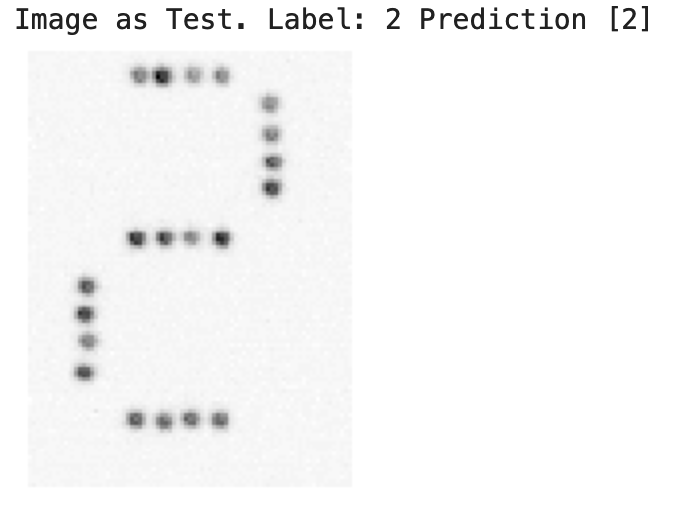
\includegraphics[scale=0.5]{pic/Prediction}
\caption{Überprüfung der Vorhersage}
\end{figure}
Außerdem wurde das Modell mit der Evaluierungsfunktion überprüft. Dazu wird das gefunden Modell mit seinen Parametern an dem Valdierungsset getestet. Dieses Datenset kennt das Modell nicht, da die Daten nicht zum Lernen verwendet werden.
Das Ergebnis war auch eine Genauigkeit von 100\%.







